%\documentclass[12pt]{report}
\documentclass[a4paper,10pt,twoside]{book}
\usepackage[DIV=14,BCOR=2mm,headinclude=true,footinclude=false]{typearea}

\makeatletter
\if@twoside % commands below work only for twoside option of \documentclass
    \newlength{\textblockoffset}
    \setlength{\textblockoffset}{12mm}
    \addtolength{\hoffset}{\textblockoffset}
    \addtolength{\evensidemargin}{-2.0\textblockoffset}
\fi
\makeatother

\usepackage[utf8]{inputenc}
\usepackage[english]{babel}
\usepackage{graphicx}
\usepackage[pdf]{pstricks}
%Options: Sonny, Lenny, Glenn, Conny, Rejne, Bjarne, Bjornstrup
%\usepackage[Sonny]{fncychap}
\usepackage{amsmath}
\usepackage{amssymb}
\usepackage[colorlinks=true, allcolors=blue]{hyperref}
\usepackage{hyperref}
%\usepackage[a4paper,top=3cm,bottom=3cm,left=3.5cm,right=3.5cm]{geometry}
\usepackage{pseudocode}

\graphicspath{ {imgs/} }
%\usepackage{natbib}

\title{
  {\Huge Inferring program structure from an execution trace}
}
\author{
  {Juan Francisco Martínez Vera}\\
  {\tt juan.martinez@bsc.es}
}
\date{\today}

\begin{document}

\maketitle
\tableofcontents

\chapter{Introduction}

On the context of this thesis and the motivations that encourage for this work.

\section{Context}
\lettrine{A}{typical} configuration for high performance machines are clusters.
It means a team of individual processors or multiprocessors 
(and lately more specific 
hardware like GPUs) working together, interconnected by a super-fast network. 
The fundamental idea behind these big machines is getting speedup by mean of
partitioning the problem and parallelize the execution. So all processors (or a 
subset) in the cluster will be dealing with different parts of the same problem 
and communicating between them in order to end up with a solution. For example 
imagine we have a weather forecast software, in order to speedup the forecast 
we can partition the surface of the earth and hold every portion to one individual
processor. The communication will be needed because the weather will also depend 
on surroundings, so every partition will need also information of other partitions 
results.

In Computer Science the discipline in charge to drive research in this field is 
the High Performance Computing, i.e. HPC. HPC has been increasing in importance 
and nowadays can be said it is the third support of science with theory and 
mathematics. The science that can be done thanks to this big machines goes from 
earthquake predictions to the analysis of the DNA of a carcinogenic cell, from
weather forecast to material physics simulation. HPC research is not just limited
to the hardware layer but drive research in all layers in the Transformation 
Hierarchy\cite{transformationHierarchy} in figure \ref{transformationHierarchyImg}.

\begin{figure}
  \caption{Levels of transformation}
  \label{transformationHierarchyImg}
  \centering
    \includegraphics[width=100px]{transformationhierarchy.png}
\end{figure}

Resources are limited and expensive, so we have to be smart and use them in an
efficient way. Improving the efficiency is not just a matter that affects to one
layer of the stack but can be applied to every one of them. For example the
tremendous evolution of the last fourty years were improvements done mostly on
circuits layer what have been following the Moore's law \cite{moore:1965}. The
manufacturers have been reducing the size of transistors by a ratio of 2 every
18 months as were predicted in figure \ref{moore-prediction}. Performance improvements 
were also at microarchitecture level with
disruptive designs that allows ILP like HPS\footnote{High Performance Substrace,
what is indeed out-of-order execution with in-order retirement.}
\cite{Patt:1985:HNM:18927.18916}, speculative execution with prefetchers, 
branch prediction or even memory access value speculation,
VLIW\footnote{Very Long Instruction Word} or TLP\footnote{Thread Level
Parallelism} with multi-threading. Improvements on memory hierarchy like cache 
associativity, non-blocking cache or trace cache. The last
big revolution affected both architecture and program layers and was the 
multicore revolution. Was specially important because until then, programmers were 
agnostics, just feel their programs went faster but now, programs have to be 
architecture aware. With this last revolution a new effort for hide machine stuff
from programmers arise and end up with programming models like OpenMP
\cite{openmp_new}, OpenACC\cite{openacc_new} or OmpSs\cite{ompss_new}. A relatively
recent example is shown is this paper \cite{Alvarez:2015:CPT:2872887.2750411}
where they are trying to automatically use the fast scraptchpad memories by
means of compilers procedures and extra hardware support instead
of let programmers to deal with this piece of hardware directly. So be 
always faster and faster is a big deal and is even more pressing in HPC because 
as it is sayd, it is fact an important science driver.

\begin{figure}
  \caption{Gordon Moore's prediction done in 1965}
  \label{moore-prediction}
  \centering
    \includegraphics[width=150px]{moore_prediction.png}
\end{figure}


This thesis is centered on program layer\footnote{The program layer 
bring together the program itself, programming models, frameworks and libraries.}. 
This layer is the actual implementation of the algorithm, i.e. where programmers
transforms algorithm to  semantic code that can be transformed lately into
executable binary by compilers. This layer is indeed the interface between pure 
algorithm and the machine architecture. Having an efficient algorithm
mathematically speaking is not enforcing having an efficient program 
because at algorithm level we do not care about the machine. 
The mechanism to assess the quality in terms of performance are the performance 
analysis tools that allows to analyze and detect the bottlenecks. 
There are two main trends, by one hand we have the profilers and by other hand trace
tools. Profiler tools generates performance summaries that provides 
coarse-grain information, with low-overhead. It means that you can feel the problem 
and infer what could be the origin but the information is not enough if you want 
to be sure. For gather more detail, the other typical approach are the tracing 
tools. High accurate and detailed information can be obtained, but it needs 
more resources in terms of cpu, disk and analyst effort because more data implies 
more complexity. This demand of resources becomes worst since the capacity in 
terms of parallelism is increasing, so the number of tasks to monitor makes 
tracing by one hand hardly scalable and by the other hand tricky to analyze
because the huge quantity of data and because the increasing response times
during the interactive exploration of analysis results. 

Researchers are currently facing this two drawbacks. There are currently several
specialists driving research in the scalability field, they are trying to reduce 
the overhead of tracing in terms of time and trace sizes by mean of several 
techniques like machine learning, data-mining and so on like in 
\cite{llort2015intelligent} or by on-line compression like in
\cite{noeth2009scalatrace}. About analysis field, the complexity of the analysis 
can be overcome by adding intelligence to performance analysis tools, last 
trend is to provide an automatic smart layer that automate an important part 
of the analysis. Some examples of this 
research line are automatic performance analysis \cite{wolf2003automatic}, 
automatic structure extraction \cite{casas2007automatic}, phases detection 
\cite{gonzalez2013application} fundamental factors models \cite{casas2008aass}, 
automatic analysis throw deep learning \cite{simon:2017:perfdp} and so on.

This thesis is focused on the analysis field and is devoted to humbly contribute 
to ease the work of the analyzers by
automate part of the analysis. The goal of this work is to automatically detect
the internal structure of an application and correlate it with performance metrics by
mean of a post-mortem trace analysis that will help to have a general
overview about what is actually going on. So instead of deal with whole
information from the very beggining, this approach let the analyzer to figure
out to what part of the gathered information focus on, speeding up the process of
analysis. Also will help to correlate performance analysis with source code
since the detected application structure would be similar as
code structure. Furthermore it will contain source code information that will allow to
easly pinpoint one metric to the code. The structure representation will ignore 
implementation details what therefore will contribute to faster and therefore better 
quality reports for developers. 

This sort of analysis have been done tipically by using sequential pattern mining
techniques what is in principle the set of techniques that better fits to this
problem since a trace is just a sequence of events ordered by time. The main
drawback of these techniques is the complexity of the algorithms that behaves
linearly in the best case and exponentially in the worst. Since the size of
traces are increasing dramatically, this problem has to be revisited. 
The main contribution of this thesis is to see structure detection problem as a 
classification problem such that non-supervised classification algorithms like 
clustering can be used taking profit of their quasi-lineal complexity in the 
general case.

% TODO: Un par de lineas sobre los resultados

% TODO
% He visto que todos los trabajos anteriores han intentado resolver el problema
% tirando de una forma o de otra de tecnicas de pattern mining. El coste de este
% tipo de algoritmos es presumiblemente alto, por lo que recuerdo haber leido de
% suele ser cuadrático. De todos modos tengo un survey sobre pattern minning que
% quiero repasar para poder atinar más sobre los costes de los algoritmos
% existentes. Esto es una motivacion desde que el tamaño de las trazas crece
% constantemente y necesitamos algoritmos más eficientes. La tesis que se
% sostiene aquí es que la detección de la estructura interna de las aplicaciones
% puede entenderse como un problema de clasificacion, es decir, clasificar los
% callstacks en conjuntos que vendrian a ser los bucles. El algoritmo por
% excelencia de clasificacion (en base a unas metricas) es el clustering, el
% cual tiene un coste, en el caso del density based clustering de casi-lineal.


\section{Motivation}

High performance computers becomes more complex every generation. The number of 
processors is increasing dramatically, e.g. the current number one on the Top500
 list\footnote{Top500 is the list of the top 500 most powerful high performance 
computers in the world. It is updated two times per year.} is the Sunway TaihuLight 
with 10,649,600 cores\cite{top500_2017} and the trend is even increment this
numbers because the exa-scale era. Analyze application with this quantity 
of processes with fine-grain detail becomes a really tough task when not
impossible because of the huge amount of information. The typical tools like 
visualizers are not enough responsiveness so one of the major challenges is the 
identification of the hot spots to just focus on these subsets of information. 
Researchers demands 
tools that ease the process of performance analysis so taking all of this into 
account the main motivation of this work is to ease the analysis by means of 
reducing execution traces to the minimal and meaningful expression.

We can say that HPC applications shares a common idiosyncrasy between them. 
Mathematic solvers needs to iterate again and again until the result converge and 
simulation software are used to be programed to evolve over timesteps. So in 
general, HPC applications consists on a big outer loop that is being executed 
again and again the same code but with evolving data, i.e. SPMD\footnote{Single
Program Multiple Data} programs. Additionally this kind of workloads are used
to be burst syncrhonous, i.e. all ranks are executing computation and
communication phases in a syncrhonous manner. For these so regular executions a
relatively simple representation of the whole execution could be extracted, i.e.
the trace could be reduced to a minimum pseudo-code expression
with aggregated data for the whole loop so its somehow folding all the iterations
space. This pseudo-code expresses indeed the actual internal structure of the 
application.

There are previous works (discussed widely on section \ref{related_work})  that 
tries to represent the internal structure of an application but they are used to
use directed graphs like in \cite{aguilar2016event} or just callstack trees like
in \cite{saviankou2015cube}. The drawback of represent the application structure
just with directed graphs is that it is a so simplified view, in the referenced
case it is impossible to pinpoint a given loop (directed graph cycle) to the
actual code because the lack of callstack information. In case of the
referenced approach that uses callstacks tree, the lack of information becomes
from the fact that there is no representation for loops (although you have fuzzy
clues like see the number of calls). The identification of this lack of clarity
on the structure representation motivates as well this thesis. The proposal is to 
generate a pseudo-code with loop and conditional structures that can be easily 
pinpointed to source code and additionally can show aggregated metrics
that will allow the analyzer to detect the interesting parts to analyze in next
steps. So it can be understood as a sort of mix of the two approaches references
above.

About the used methodology, it can be considered a disruption in this field. The
previous proposals are used to drive this problem using pattern mining
techniques (the basic idea of these algorithms are exposed on section
\ref{pattern_mining}). That is the obvious choice because a trace is basically a
sequence of events sorted by time. The problem with these sort of algorithm are
the complexity. So the last motivation is about reducing the complexity. 
Taking into account the exponential increassing of traces sizes 
this thesis contribution is the idea to perform intern structure analysis 
instead of as a pattern mining problem, as a classification problem. 
Classification algorithms like clustering presents much better performance with 
about quasy-lineal costs.

%\section{Performance analysis tools environment and workflow}\label{s:pt_evironment}
\section{Performance analysis tools}\label{s:pt_evironment}

This thesis has been developed in the Performance Tools team at Barcelona
Supercomputing Center and therefore the tool and techniques explained in this
document have been designed to fit in this environment. 

The main tools designed and developed in the BSC Performance Tools Team are 
Extrae, Paraver and Dimemas although other satellite tools are also in the environment they will not be
explained because are out of the scope of this project. These tools are: 
Clustering, Tracking, Folding, Spectral and Basic Analysis.

\subsection{Extrae}

Like it name (in spanish) indicates, it is about extracting information. Extrae is
the piece of software in charge of inject monitors to the application to
be studied and
extract valuable information for the analysis. Different mechanism for
monitoring are available being the most used the interposition mechanism by
means of the {\tt LD\_PRELOAD} environment variable present in UNIX systems.
By this mechanism just calls to a given framework can be instrumented because
what it does is to divert a framework calls by the program to extrae, then extrae get
the information and calls the actual framework function. It supports several frameworks: 
\begin{enumerate*}[label=(\roman*)]
  \item MPI (for several implementations)
  \item OpenMP
  \item OMPSs
  \item CUDA
  \item OpenCL
  \item pThreads
  \item Java
  \item and Python.
\end{enumerate*}

The information that can be collected by Extrae is not just timming what is maybe
the most important one but also some hardware counters by means of PAPI
interface. All of this information can be complemented by user events that can
push the desired information to the tracefile by means of the Extrae API. One
possible use of the Extrae API is to extract information about how different
iterations from a given loop are behaving.

All these gathered information from all threads/processes in the target
application is finally merged and presented to the analizer as an ASCII
tracefile. Since the task of analyze a super-huge ASCII file is a tough work, a
visualizer has been developed, that is Paraver.

\subsection{Paraver}

The task of analyze numbers is tough when there is a huge quantity so
the natural choice is to represent them visually since we as humans are very
good understanding visual patterns. For example in mathematics
is usual to use plots. In the field of performance analysis, visualizer tools
also has been developed, having in BSC the Paraver tool that as its name indicates
(in spanish) is  about ``to see''. Paraver allows to have a qualitative global 
perception of the application behavior by visual inspection and then to be able 
to focus on the detailed quantitative analysis of the problems.

Its power lies on two main concepts. The first one is that paraver traces are
semantic agnostics therefore it is provided by auxiliar files called pcf (paraver
configuration file\footnote{Do not confuse with cfg files}) and row\footnote{It 
is called row because it provide names for the rows of the timeline so for the 
space axis} (names configuration file). It allows to extend the tool with
support for new performance data or programming models easily. The second and
more interesting is that the derived calculations from initial metrics from trace is
not hardcoded in the tool but configurable so for example to derive a typical
metric like IPC you should filter number of
instructions by one hand, number of cycles by the other hand and then perfom a
division. This powerful approach give the resposability to the user that can
leads to the ``blank page
syndrome''\footnote{https://en.wikipedia.org/wiki/Writer\%27s\_block\#Blank\_page
\_syndrome} for the not so skiled users. For avoid this
sort of problems the Paraver package provides a set of configuration files of
the most used views that perform all the filters and derivations for you.

\subsection{Dimemas}

Like the other tools Dimemas also have a so descriptive name, it means (in
spanish) ``tell me more'' but is fine to use the acronim that is ``DIstributed
MEmory MAchine Simulator''. It is a high-abstracted trace-driven MPI simulator
perfect to perform the called ``what if'' experiments. It is capable to simulate
the interconection network of a distributed memory machine by means of a high
abstracted model that consists on three fundamental parameters:
\begin{enumerate*}[label=(\roman*)]
  \item Latency (s) that models the actual latency of the network and also the
    possible overhead because the software stack before arrives to the NIC
  \item Bandwidth (mb/s) that models the bandwidth of the network and
  \item Contention that is modeled by the number of messages in flight 
    allowed on a given instant on a given network (intra-nodes, inter-nodes or
    inter-machines) and the number of input and output messages from a given
    node in a given instant.
\end{enumerate*}

Dimemas as Paraver is Extrae-dependant software since they need traces to work.
In the Dimemas case it needs to perform a conversion by means of the {\tt
prv2dim} converter in order to ease the simulation. As an output it builds up a
new Paraver trace that can be analyzed as the original.

Only communication times are simulated through the Dimemas models so CPU times
remain the same on the output tracefile. Even if it is a minor detail, since it
is important to introduce because the usefulness of it for the purposses of this
thesis, actually there is a mechanism to modify CPU burst times. At parsing time
(done by the {\tt prv2dim}) a hardware counter and a coeficient to multiply 
for this it can be specified. Normally the hardware counter is the number of 
cycles and the coeficient is the cycle time. By this way the user is able to 
remove the possible O.S. noise that has affected the original
execution\footnote{Noise intruced by O.S. can be detected in Paraver by a fall 
  of the frecuency. This is becuse cycles counter forms part of the context of
  every process but not the time so whenever a process loss CPU, cycles will not
  be counted until return to execution but time is not stopped although. This
  phenomena implies an increment on the traced cycle time. Take into account
  that is impossible to guarantee a fall on frequency is because O.S. or because
  any other source like DVFS so it works only when we can assume the frequency
of the processor is quite stable.}.

\subsection{Analysis workflow}

In an application-centric
approach, the performance analysis is a cyclic process consisting of observing 
the behaviour of the application so as to hypothesize the possible problems 
that affect its performance and finally translate these hypotheses to 
improvements in the application re-starting the cycle to validate them as is
depicted in figure \ref{fig:perf_analysis_workflow}.
Obviously, the less number of iterations of this cycle the less time wasted and it directly depends on the quality of the hypothesis that is strongly related with the possibilities the analysis tools provides.

\begin{figure}[]
  \centering
  \includegraphics[width=150px]{performance_analysis_diagram.png}
  \caption{Performance analysis workflow}
  \label{fig:perf_analysis_workflow}
\end{figure}

\begin{figure}[]
  \centering
  \includegraphics[width=80px]{analysis_subphases.png}
  \caption{Analysis subphases}
  \label{fig:analysis_subphases}
\end{figure}

This work is centered on the analysis phase of the workflow and more accuratelly on
the initial phases of the analysis where all the non important information is
tried to be filtered and rejected in order to work with these regions of
interest from where more valuable information can be gathered. The current
approach is  a craftwork where the experience of the analyzer is crucial to have
a good quality results since this is not an easy task because information 
obtained from the trace extraction phase used to be huge. Analysis phase is
typical subdivided into the following subphases (see figure
\ref{fig:analysis_subphases}):
\begin{enumerate}[label=\roman*)]
  \item Filter as much as possible irrelevant information. Before this phase is
    used to be impossible to work with visualizers so the main goal is to end up
    just with the needed information for inspect the structure of the
    application.
  \item HPC applications are used to have a common idiosincracy that is to
    present very repetitive patterns both in space (different processes) and 
    time dimensions. Exploiting this typical characteristic, next step is cut
    the more interesting parts of the execution e.g. an iteration or a set of
    iterations that seems to presents interesting information because its 
    extremelly bad performance.
  \item Last and most important, the analysis. Once one part of the execution is
    detected to be interesting it is then gathered from the original trace i.e.
    with all the original information.
\end{enumerate}
This work could be very difficult and tedious and used to drive to repeat the
same process several times and since every one of the steps is potentially very 
time consumed when dealing with huge trace, it could be a waste of time. Both first and second subphases could need to be repeated
several times because the first filter is not good enough or because on the last
phase analyzer realize the cut is not as interesting as looked like.

Summing up there is a lot of repetitive craftwork that can be and even have to
be automatized leading the work more efficient and effective, making available
more time to the actual real work that is figure out what is going on with the
performance that is the imaginative and human work. In this thesis this problem
has been identified and studied and is trying to solve it by proposing
an alternative way to deal with analysis phase. As has been introduced before, 
the proposal consist basically 
on instead of playing and try to figure out what to filter what to cut and what
to analyze, ease this process by providing the minimal and meaningful expression
of the trace, transforming it to a pseudocode with performance information 
attached that will leads to an easy decission to what to analyze first.

\chapter{State of the Art review}

\section{Previous and related work}\label{related_work}

\lettrine{T}{he problem} of the analysis scalability is not faced for the first time in 
this paper but there is a previous work in what this thesis is rely and is 
supported on. Several tools are actually being used in order to ease the analyst
work. Talking about structure analysis we can split previous works into two main
subsets. By one hand we have the behavioral structure that want to expose the
different phases on an execution in terms of performance and by the other hand
the syntactic structure that provide information about the actual program
structure such as profiling.

\subsection{Behavioral structure}

If we consider the same bunch of code will behave, in general, in the same
manner it can be assumed that there is a powerful correlation between the
behavior and the code. By this way it can be said a behavioral analysis is a
side-channel analysis because indirectly the internal syntactic structure can be
betrayed. This consideration could be true in some cases but not in general. The 
main goal of the different approaches presented in this section is not
to present a syntactic but a behavioral structure. The motivation is that when
analyst deals with syntactic structure, time variations of the same functions is
hidden. This situation can appears for example when calling same function with
different parameters. For the analyst point of view could be more interesting to
have this information unfolded. Take into account that this same property can
end up identifying different parts of the code as the same phase.

Even if the goal of the approaches explained below does not match perfectly with
goal of this thesis, they provide a really useful insights as a related work.

In \cite{casas2007automatic} they propose, similarly to this paper, 
automatically extract the internal structure of an MPI application from a
Paraver tracefile and provide to analyst just representative phases. 
They rely on signal analysis for this propose. 
Their analysis consists on two main phases:
The first is to clean-up the trace by identify the perturbed regions.
Perturbed regions are those parts of the trace that has been perturbed nor by
the application nor by architecture but by external factors such that unknown
system activity or tracing package. Their clean-up phase is centered on remove
noise from tracing package, i.e. flush to disk. By building up a signal based
on flushing events and transform it by Closing morphological filter they end up
with this perturbed phases. The second phase is the identification of the
phases. It is done by means of autocorrelation and periodicity analysis of a
signal. This signal is build up from any metric like instantaneous FLOPs but the
use number of MPI point to point calls being executed. Once the period is
successfully detected the same process is done recursively on one of the
periods. This allows to have a hierarchical structure. Finally the output is
basically information about the different phases like number of iteration and
timing plus some representative cuts of the original trace. It differs on this
thesis approach basically on the fact that they extract the structure by
behavioral analysis instead of actual callstacks analysis. The main drawback is
this method is not concerning about noise from the actual application so same
phase on code can be detected as different phases, also if there is a lot of
perturbation at level of e.g. cache, depending on what metric is being used, no
structure could be detected. 

Similarly with the previous approach, in 
\cite{gonzalez2013application} is proposed to apply clustering techniques in
order to identify the different execution phases. Different parts of the
execution are considered as the same phase depending on the behavior,
so an analysis using some hardware metrics is
performed. The first phase is about reducing the complexity of the clustering by
filtering the less relevant computation burst, i.e. little bursts according
with a given threshold. In order to reduce the dimensionality the proposal is to
use two different dimension sets: The first one is Completed Instructions
against IPC\footnote{Instructions per cycle}. This configuration provides a
performance view. The second is Completed instructions against L1 and L2 cache
misses. This combination reflects the impact of the architecture on the
application structure. 

\subsection{Syntactic structure}

Syntactic structure is centered on providing the actual program code structure so
it needs to use some debug information about symbols and about the position of
the instruction in code is being executed and monitoring, i.e. the callstack.

The main interest on having the syntactic structure of an application is to be
aware about not just what but where. This is important in the process of who to
blame in code and provides insights of the actual application that with just
behavioral structure can not be presented like for example where do we have
loops and how many iterations performs.

Profile tools are used to present behavior information attached to a 
syntactic structure. Although this is a scalable
solution for performance monitoring, they are used to discard temporal order so
structures like loops are just exposed indirectly by the number of calls metric.
Additionally some sort of bottlenecks like late-sender problems are difficult to
detect without time order information. These following approaches presents the
information in a way that are in the midway between profilers and tracers. In
general starts from a huge trace and by means of summarizing and aggregating
data tries to present the minimum and meaningful information to the analyst.

In \cite{noeth2009scalatrace} they are concerning about the scalability of the
tracing part. Even if they are centered on the logging (or tracing) part their
work is really useful for this thesis purposes. They claim reductions of about a
thousand in terms of trace size just by detecting the structure of the
application, e.g. If the same thing is repeated 100 times, just saving it once
and tagging with the number of times it is executed should be enough. They
propose to use RSD (Regular Section Descriptors) to express MPI events nested
inside a loop and a sequence analysis algorithm loosely based on the SIGMA
scheme for memory analysis for detect the repetitive patterns. Their compression
is done in two phases. The first one is an intra-node compression, where the
repetitive patterns arise and the second one is inter-node merge, where all
single-node compressions are merged forming the whole application trace.
They introduce interesting concepts as calling sequence identification used for
unambiguously identify different MPI calls that lie on different code positions, 
and recursion folding signatures for dealing with recursion. Also they claim
that even if their main target is to compress traces, Scalatrace also can be
used for analyze the application structure by doing a little demo showing how it
can detect the most outer loop iterations or timesteps. One of the main
drawbacks of this approach is that the complexity of both intra-node and
inter-node compression can be of $O(n^2)$.

In the same line as the previous work, Compressed Complete Call Graphs (cCCG) are 
presented by \cite{knupfer2005construction}. It is about finding repetitive 
patterns for loosely or lossless compression but instead of at tracing time, 
over an already traced huge trace. 
This compression will allow to analyst to analyze whole huge traces 
interactively, difficult business when dealing with this amounts of information. 
CCG is basically a graph of function calls of a program so the main structure is
defined by the function call hierarchy while additional information are appended
usually as leaf nodes. The construction phase is quite simple. The trace is
traversed in a sequential manner, every time a function enter event is detected,
new node is generated and append to the current active node. The
other way around when exit function event is read, the current active node is
finalized and all information concerning to this node is presented e.g.
duration. Additionally, while constructing, the graph is compressed. The basic 
idea is to replace $n$ repeated sub-trees that are equal or similar with a 
reference to a single instance saving $n-1$ remaining copies. For similar is
understood that when comparing nodes not all properties must be equal for
example is not needed some scalar values like duration match perfectly (some
configured deviation is acceptable) but properties like function id must. They
claim main compression ration about 200 can be achieved with this approach.
Additionally this compression technique does not need to uncompress anything, the
user (or any analysis algorithm) just can traverse the graph and gather
information.

This approach improves profiling in the sense that same function with same call
path and different time behaviour is exposed to analyst but still presents a lack 
of information on the order of the execution of the different graph paths.In
\cite{aguilar2016event} they present the Event Flow Graphs (EFG) as an intent of
provide temporal order between events. In this case they are centered on
syntactic structure but just focused on MPI operations. EFG are
weighted directed graphs where every node is an MPI call and edges the
transitions between them, so the program code blocks executed between them.
Graph nodes can contain aggregate information like call duration or message size
and edges can be attached with information about CPU burst like performance
metrics like IPC additionally to the number of times the edge is traversed.
Now let's imagine we have a loop where there are three MPI calls $A$, $B$ and
$C$ and $B$ and $C$ are mutual exclusively executed so if we have 10 
iterations we have $A*10$, $B*5$ and $C*5$. In order to reconstruct the execution
we need information about in what iterations B and C have been executed.
So additionally they present temporal-EFG that introduce more
information for these cases where the execution order can not be reconstructed
with the previous EFG. They claim this technique can be used for trace
compression, application structure detection and visual performance analysis.
Following with application structure detection, what is where this thesis is
focused on, they use algorithms for cycle detection over the t-EFG (DFS-based)
and once cycles are detected the graph is transformed to a hierarchical tree
where loops and subloops are showed up. Statistics about loops can be gathered
like number of iterations, total time in loops and so on.

Even if they use code position information for building up they EFG (as it can
be seen in previous publication \cite{aguilar2014mpi}) they are not pushing it
to analyst so it is not clear how they are relating EFG with source code for the
analysis.

In \cite{trahay2015selecting} they present an approach for select points of
interest automatically, understanding as points of interest these iterations that
behave different from the majority. The first phase is a post-mortem analysis of
a given trace. This analysis is about finding patterns of events that are
repeated, i.e. folding loops that has been unfolded during the
tracing\footnote{Unfolding in the sense that tracing process represent loops as
a sequence of a repeated set of events.}. Their algorithm is about finding short
repeated sequences of events and try to expand the pattern. After detect the
intern structure of an application, the distribution of durations of the
different iterations of the detected loops is an arbitrary construction, so they
is this construction in order to filter all iterations that behave similar and
expose to analyst these iterations that are outliers assuming these ones are the
most interesting ones.

Unlike other works, this last work is not presenting any visualization of the
structure to the user. Also they are not relying on the idea of signature in
terms of all the call path for comparing events but instead they define two 
events to be equal if they enter or leave same function and have exactly the
same properties. Imagine that we have two processes, the first one is sending a
vector of size $N$ in chuncks of $m$ having $N\:mod\: m \neq 0$. One of the messages
will be different on size but is exactly the same send in terms of position in
code. The proposed algorithm will detect two different patterns here. The
problem is worst when dealing with more unstable algorithms.

Next approach is about “profilization” of traces.
In \cite{saviankou2015cube} 
\dots

\section{Performance analysis tools environment and workflow}\label{s:pt_evironment}

%\begin{figure}
%  \caption{Current performance analysis workflow}
%  \label{currentAnalysisFlow}
%  \centering
%    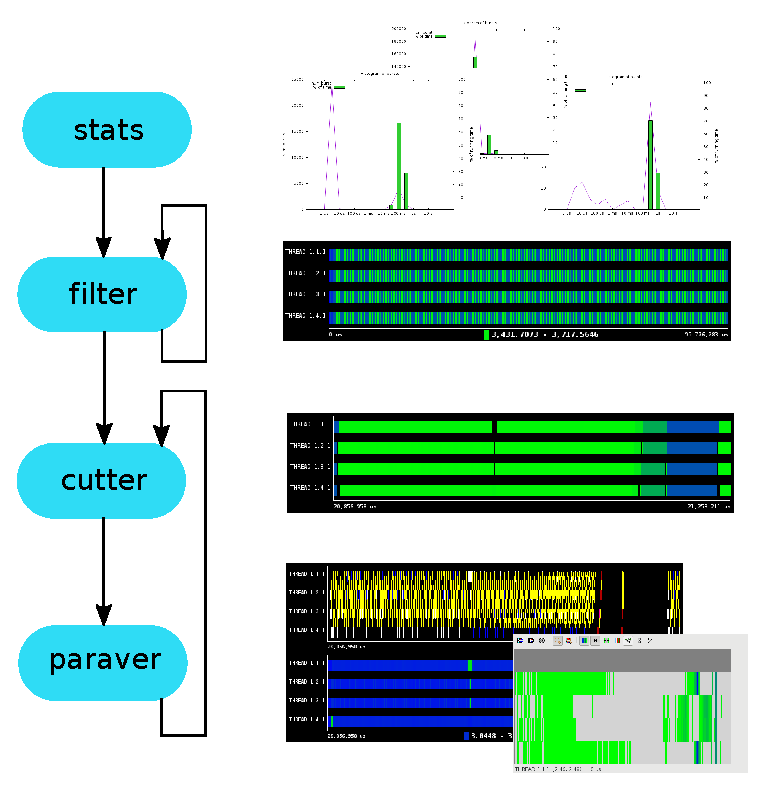
\includegraphics[width=250px]{current_analysis_flow.eps}
%\end{figure}

Talk about the BSC performance tools environment and introduce the analysis flow
with and without this proposed tool.

This is the mission of the parallel performance analysis. In an application-centric
approach, the performance analysis is a cyclic process consisting of observing 
the behaviour of the application so as to hypothesize the possible problems that 
affect its performance and finally translate these hypotheses to improvements in
the application re-starting the cycle to validate them. Obviously, the less number 
of iterations of this cycle the less time wasted and also the less money spent.


% NOTES
% .- Remember to demonstrate the interarrival time of different calls in the sam
%e loop body tend to be the same.




\chapter{Scalable structure detection}

On the previous studies and the proposed methodology

\section{Previous studies}

Before entering to the description of the actual tool development, in this 
section it is going to be explained the previous studies that have been done and
have driven to the taken decisions.

\subsection{Application structure by classification}

Taking into account the motivations, exposed in \ref{s:motivations}, and the
previous works studied and discussed in \ref{related_work} the idea to introduce
a new approach arise, even if as always based on previous foundations.  
 
Our intention is, in principle, just use information from MPI calls, mainly for 
three reasons:
\begin{enumerate*}[label=\roman*)]
  \item It does not needs to instrument the source code of the target
    application since exploit the \texttt{LD\_PRELOAD} capabilities of extrae.
    It is a big deal since the source code is not always available to the
    analyst.
  \item trace size is small compared with traces with more information
    like entry/exit from functions
  \item and as have been argued in \ref{s:soa_discussion} monitoring the MPI 
    calls is enough for having a clue about the general structure of the 
    application.
\end{enumerate*}

The proposal presented in this thesis is to explore a new way to detect the
 general structure of an application by applying clustering. 
The essential point is that the problem has been converted in to a classification 
problem so instead of looking for these itemsets that are being
repeated several times during the execution, close enough one each other, let's
face the problem of arrange the MPI calls that belongs to the same loop to the
same cluster. Then analyze the hierarchical arrangement of these clusters to
detect superloops-subloops relations. Once done, the pseudo-code representation 
construction becomes quite easy. The scalability of this method resides on the 
fact that
HPC applications are strongly repetitive over the time, so the number of unique
MPI calls to cluster remains about constant despite the growth of the execution
time, additionally clustering algorithm such that K-means presents an attractive 
linear complexity and DBSCAN a quasi-lineal in general.

The two previous studies that follows in this section are 
\begin{enumerate*}[label=\roman*)]
  \item since we want to group MPI calls into loops, is important to know what
    is actually identifying a loop
  \item and perform a quantitative demonstration of the scalability of the
    method in terms of number of unique MPI calls for different growing inputs.
\end{enumerate*}
Both studies have been done over executions of the MPI NAS Parallel benchmarks 
in its 3.3 version.

\subsection{Loops feature selection}\label{ss:loops_characterzation}

The key point of the presented method is to clustering MPI calls into loops but
what is actually identifying a loop? The answer is about to figure out what loop
feature or features are able to identify then unequivocally or at least with
less level of aliasing\footnote{Understanding as aliasing when two different
loops are considered the same because impossibility to differentiate throw the
selected metrics}. Without a lot of 
effort we can think that its
position on code, understanding as position the line and the file where the loop
lies, is the feature that will give us more information but the reality is that 
we do not have this information on trace. To have it we would need to insert
some monitors on code or maybe use some sort of dynamic binary instrumentation
like
PIN\footnote{https://software.intel.com/en-us/articles/pin-a-dynamic-binary-instrumentation-tool}
and it would drive to huge traces, a thing to be avoided so we just are going to
rely on {\tt LD\_PRELOAD} that only trace MPI calls with additional
information like its parameters, the call-path and some hardware metrics (even
if it is true that there is also no information about loop iterations in trace,
the MPI calls repetition can be considered as a proxy of iterations)
Being aware of that, the next obvious metrics that in principle can characterize 
a loop is the number of iterations it performs but for sure in an application 
there used to be dozens of
loops and is not ridiculous to think that clustering just with this metric will
leads to a lot of aliasing. That would be true if we think in static number of
iterations but lets think about dynamic number of iterations: The dynamic
iterations of a given loop does not depends only on the number of iterations in
its definition but also on the number of iterations on the definition of the
parent loops such that if there are two loops having $n$ and $n$ iterations (so
having aliasing on static number of iterations) being one nested on the other, 
in the dynamic domain, they will have $n$ and $n^2$ iterations, undoing the aliasing.
This is just an starting point, nested loops will be unambiguously identified so
it is okay for most of the applications (the most simple) but there still some
situations where we can have aliasing. The situation where two loops
lies on the same loop nesting level and have the same number of static
iterations will drive to aliasing. This situation is not so probable (at least
on the NPB benchmarks that is the set of benchmarks used for validation) but
since it has been detected in some cases it has to be covered. Further, the next
metric that can identify a given loop is the work that does, i.e. the
iteration time. Two different loops used to execute different work so it is
likely to have a different duration per iteration. An appropriate metric for
quantify this value is to take an aggregate of all iterations duration, i.e.
the mean. So, in this first qualitative approach, the conclusion is we can 
identify with high probability of 
unambiguity the loops with two metrics:
\begin{enumerate*}[label=\roman*)] 
  \item Number of dynamic iterations
  \item Iterations mean time
\end{enumerate*}

Additionally to this qualitative discussion, it is crucial to drive also a 
quantitative analysis. In order to do so, 
several features, the described above and some others, are collected from several 
executions and a feature selection is then done by means of two well-known methods
\footnote{Feature selection is
the process of selection a subset of relevant features for use in the model
construction.}.
The main objective is to confirms or reject our intuition about number of
iterations and iteration mean time, and to find out other possible features that
can help on the task of identify loops.
The first used technique is PCA analysis that permit to get hints 
about how features are related between them and the last is a variable 
importance analysis by means of Random Forest method. On next sections will be 
explained how data have been gathered and the analysis performed over it.  

\subsubsection{Data acquisition}

Previously have been discussed how number of dynamic 
iterations and iterations mean time can help. Additionally to these information
\begin{enumerate*}[label=\roman*)]
    \item IPC 
    \item and some instruction types counters 
\end{enumerate*}
will be also gathered.
About the former, we would need mean number of instructions and mean number of 
cycles per iterations. The reason is that they maybe can contribute because some 
differences in the performance between loops. The intuition says that
hardly can help for this purposes because, among other reasons, it depends a lot
on other factors than the application. Remember in previous sections have been argued
performance information is not optimal for syntactic analysis but we can not
discard it categorically before do a quantitative analysis. The reason for the
latest is that it can be thought if two loops performs different work, the
relative quantity with total number of instructions of scalar, floating point 
or memory operations will differ. In order to do so, a set of hardware
counters have been defined. The decision about what hardware counters
pick have been dramatically restricted because the capabilities of the
hardware used for the experiments. This set consist on:
\begin{enumerate*}[label=\roman*)]
  \item Number of instructions
  \item number of cycles 
  \item number of unconditional branches
  \item number of conditional branches 
  \item total number of branches
  \item number of floating-point instructions
  \item and number of memory loads.
\end{enumerate*}
Finally we also want to collect an unambiguously identification of loops
since we want to be able to accurately relate these metrics to a given loop.
The identification is done by hash function with code line and file.

As has been introduced above, trace does not have explicit information about 
loops so it should be collected from other sources. The reason is that the typical
tracing method is by means of the {\tt LD\_PRELOAD} mechanism, so tracer library just
can get information at shared library calls (like MPI, GOMP, \dots). The alternative
is to manually instrument the user code and fire events with the desired information
by means of the tracer library API, in this case Extrae. Since the process of
manually insert monitors presents to be tough for large codes has been decided
to do it automatically using a source-to-source compiler, in this case
Mercurium. Modifications on Mercurium have been done what have consisted
basically on develop a new compilation phase that injects the desired
monitors on the desired places in the code. Now, at execution time, those
monitors  fires the desired information to trace. 
All developments for this purpose are explained in annex \ref{ann:automatic_loops_charac} 
in more detail.

Slightly different approaches have been applied in every case. In the case of
the PCA, since we wanted to characterize loops as a single entity, events are
fired at the beginning and at the end of every loop marking the loop boundaries
with just loop identification information, furthermore also events are fired at 
the beginning and at the end of loops iterations, in this case with all the
mentioned hardware counters. Since tracefile presents to grow to dozens of
Gigabytes for not so big executions and executions tends to be really stable
just picking several iterations seems to be enough, so have been decided to 
instead of instrument all iterations of all loops, an iteration is instrumented 
given a probability. For these experiments the probability was set to 20\%.
Finally to keep track of how many iterations has been instrumented over the
total, an extra event with total number of executed iterations (instrumented or
not) is also fired to trace for every loop.

For random forest analysis data acquisition is done from another perspective, 
in this case what we wanted is the same information that will be available on
production traces but labeled with the information of to what loop it belongs
to, so these traces can be understood as training  traces. To do so the
functions that marks entry/exit of loops does not fire any event to trace but
keep track of the loops nesting hierarchy. Loop identification (or
identifications when in a nested loops) is only fired to trace before an MPI call. 

After data have been gathered to traces, post-process is done for
prepare it for the performed analysis. On next section will be explained 
how this data have been analyzed by means of the two selected methods. 

\subsubsection{Data analysis}

The first selected technique to drive the
analysis has been the Principal Component Analysis (PCA): Data is linearly 
transformed in such a way it can be expressed in principal components that are 
sorted by the amount of variance that can explain and are orthogonal between 
them. It allows to identify patterns in data and expressing the data in 
such a way to highlight their similarities and differences. Once these patterns 
are found data can be compressed by reducing the number of dimensions with not 
much loss of information.  For improve
understandability of the PCA, Variable factor map is used: It
presents a view of the projection of the observed variables projected into the
plane spanned by the first two principal components. This shows us the
structural relationship between the variables and the components. The projection
of a variable vector onto the component axis allows us to directly read the
correlation between the variable and the component.

What we wanted to see through the PCA analysis is what features can better
identify loops. To do so what is presented as input to the PCA procedure is a
set of observations that are the loops with a set of features for every one of
them. To prepare the data in this terms, a post-process of traces have been
done. This post-process have consisted on aggregate all information from different
iterations for every loop. This aggregation have been basically perform a
geometrical mean of the gathered features minus for the special case of the
number of iterations. In this last case total number of iterations is not the
total number of instrumented iterations because not all of them have been
instrumented but just a subset. Since the probability of an iteration to be
instrumented is well-known (it has been set by us), the reconstructions is also
trivial, being the total number of iterations:
$$
nit = iit*\frac{1}{\alpha^{\beta+1}}
$$
Being $\alpha$ the probability to be instrumented and $\beta$ the nesting level
of the loop.

After acquire and process the data, at image \ref{fig:sp_pcv_hwc2} it can be
seen the contribution to the variance of every principal component for every NPB
execution. In image \ref{fig:sp_pcv_hwc1} the different variable factor maps are
showed up. About the former just comment that the first principal component can
explain the majority of the variance having a value from about 70\% to above
80\% for the EP case (\ref{fig:ep_pcv_hwc2}). Moving on, the last figure is 
showing us how the variables are correlated between them and also how they are 
correlated with the components. A more detailed analysis have to be done here.

\begin{figure}
    \centering
    \begin{subfigure}[b]{0.3\textwidth}
        \includegraphics[width=\textwidth]{pcas/bt_A_4_pvar01.png}
        \caption{BT}
        \label{fig:bt_pcv_hwc2}
    \end{subfigure}
    \quad
    \begin{subfigure}[b]{0.3\textwidth}
        \includegraphics[width=\textwidth]{pcas/cg_A_4_pvar01.png}
        \caption{CG}
        \label{fig:cg_pcv_hwc2}
    \end{subfigure}
    \quad
    \begin{subfigure}[b]{0.3\textwidth}
        \includegraphics[width=\textwidth]{pcas/ep_A_4_pvar01.png}
        \caption{EP}
        \label{fig:ep_pcv_hwc2}
    \end{subfigure}
    
    \begin{subfigure}[b]{0.3\textwidth}
        \includegraphics[width=\textwidth]{pcas/ft_A_4_pvar01.png}
        \caption{FT}
        \label{fig:ft_pcv_hwc2}
    \end{subfigure}
    \quad
    \begin{subfigure}[b]{0.3\textwidth}
        \includegraphics[width=\textwidth]{pcas/lu_A_4_pvar01.png}
        \caption{LU}
        \label{fig:lu_pcv_hwc2}
    \end{subfigure}
    \quad
    \begin{subfigure}[b]{0.3\textwidth}
        \includegraphics[width=\textwidth]{pcas/mg_A_4_pvar01.png}
        \caption{MG}
        \label{fig:mg_pcv_hwc2}
    \end{subfigure}

    \begin{subfigure}[b]{0.3\textwidth}
        \includegraphics[width=\textwidth]{pcas/sp_A_4_pvar01.png}
        \caption{SP}
        \label{fig:sp_pcv_hwc2}
    \end{subfigure}
    \caption{Principal Components variability explanation}
\end{figure}

\begin{figure}
    \centering
    \begin{subfigure}[b]{0.3\textwidth}
        \includegraphics[width=\textwidth]{pcas/bt_A_4_varmap01.png}
        \caption{BT}
        \label{fig:bt_pcv_hwc1}
    \end{subfigure}
    \quad
    \begin{subfigure}[b]{0.3\textwidth}
        \includegraphics[width=\textwidth]{pcas/cg_A_4_varmap01.png}
        \caption{CG}
        \label{fig:cg_pcv_hwc1}
    \end{subfigure}
    \quad
    \begin{subfigure}[b]{0.3\textwidth}
        \includegraphics[width=\textwidth]{pcas/ep_A_4_varmap01.png}
        \caption{EP}
        \label{fig:ep_pcv_hwc1}
    \end{subfigure}
    
    \begin{subfigure}[b]{0.3\textwidth}
        \includegraphics[width=\textwidth]{pcas/ft_A_4_varmap01.png}
        \caption{FT}
        \label{fig:ft_pcv_hwc1}
    \end{subfigure}
    \quad
    \begin{subfigure}[b]{0.3\textwidth}
        \includegraphics[width=\textwidth]{pcas/lu_A_4_varmap01.png}
        \caption{LU}
        \label{fig:lu_pcv_hwc1}
    \end{subfigure}
    \quad
    \begin{subfigure}[b]{0.3\textwidth}
        \includegraphics[width=\textwidth]{pcas/mg_A_4_varmap01.png}
        \caption{MG}
        \label{fig:mg_pcv_hwc1}
    \end{subfigure}

    \begin{subfigure}[b]{0.3\textwidth}
        \includegraphics[width=\textwidth]{pcas/sp_A_4_varmap01.png}
        \caption{SP}
        \label{fig:sp_pcv_hwc1}
    \end{subfigure}
    \caption{Variable factor map on NPB with both HWC merged}
\end{figure}

First thing to analyze is whether the first qualitative considerations done at
the very beginning of this section were true or not. About total number of
iterations it can be seen that is the variable better correlated to the 
second principal component in \ref{fig:bt_pcv_hwc1}, \ref{fig:cg_pcv_hwc1},
\ref{fig:ft_pcv_hwc1} and \ref{fig:lu_pcv_hwc1}. In case of
\ref{fig:ep_pcv_hwc1} it is important for first and second PC. About mean 
iteration time it can be seen is highly correlated with first component in
\ref{fig:cg_pcv_hwc1}, \ref{fig:ep_pcv_hwc1} and with the second in
\ref{fig:ft_pcv_hwc1} and \ref{fig:mg_pcv_hwc1}. Both seems to be quite
important in general so the first intuition was not bad at all. The bad news are
that both metrics used to maintain a high correlation between them, in general
negative, what is saying as more (dynamic) iteration a loop has, less iteration
time. It have two lectures:
\begin{enumerate*}[label=\roman*)]
  \item It can be understood because the big loops that drives the execution are
    expensive because does a lot of computations and little function loops with
    simple jobs performs a lot of iterations like for example functions that
    looks for a character in a string.
  \item The other lecture is that since we are counting dynamic iterations,
    subloops for sure will have more iterations that the big outer loops and
    also the iteration time for those big loops is inevitably bigger because
    they are containing those subloops.
\end{enumerate*}
Nevertheless there are some situations where this correlation is not like in
\ref{fig:cg_pcv_hwc1} and \ref{fig:ep_pcv_hwc1}  where they are orthogonal. The
conclusion is that these two metrics can explain a quite good amount of
variability and can avoid aliasing in some cases so the first intuition seems to
be good.

Next thing to analyze is whether the IPC can help at the
classification step mostly on cases where number of iterations and iterations
time are highly correlated that happens more obviously on \ref{fig:bt_pcv_hwc1},
\ref{fig:ft_pcv_hwc1}, \ref{fig:lu_pcv_hwc1} and \ref{fig:mg_pcv_hwc1}. In these
cases it is used to present a moderated positive correlation with iteration mean
time so better IPC when longest iterations. With this data the usefulness or not
about IPC metric is fuzzy so more analysis needs to be done.

Lastly for PCA, it needs to check out how the instructions types counters are
behaving. About branch instruction counters (PAPI\_BR\_UCN\_REL,
PAPI\_BR\_UCN\_REL and PAPI\_BR\_UCN\_REL) it can be said that in general they
are strong positive correlated between them, presents a strong
correlation with first component and is used to be orthogonal with iteration
time mean and total number of iterations in cases when they are strongly
correlated. What it means is that it can explain a lot of variability of the 
dataset. Additionally since all three are explaining the same picking just one
should be enough. About the relative number of load instructions 
(PAPI\_LD\_INS\_REL) it presents a quite different behavior depending on the
execution but in most cases it presents a negative correlation with number of
branches like in \ref{fig:bt_pcv_hwc1}, \ref{fig:cg_pcv_hwc1},
\ref{fig:ft_pcv_hwc1} and \ref{fig:mg_pcv_hwc1} what means that in most cases it
can be used as well as branch counter when there is high correlation between
total iterations and iterations mean time. Lastly, about relative floating
point instructions (PAPI\_FP\_INS\_REL) like before its behavior differs
depending on the execution with respect to the rest of metrics but it is true 
that can explain quite a lot of variance.

% TODO PCA Conclusions
Summing up, \ldots


The second used technique have been random forest for classification
% TODO: Explicar Random Forest
% TODO: Explicar para que lo queremos
% TODO: Explicar el post-proceso de los datos
% TODO: Explicar los resultados
% TODO: Conclusiones

In figure 

\begin{figure}
    \centering
    \begin{subfigure}[b]{0.3\textwidth}
        \includegraphics[width=\textwidth]{varimp/bt_A_4_varimp.png}
        \caption{BT}
        \label{fig:bt_varimp}
    \end{subfigure}
    \quad
    \begin{subfigure}[b]{0.3\textwidth}
        \includegraphics[width=\textwidth]{varimp/cg_A_4_varimp.png}
        \caption{CG}
        \label{fig:cg_varimp}
    \end{subfigure}
    \quad
    \begin{subfigure}[b]{0.3\textwidth}
        \includegraphics[width=\textwidth]{varimp/ep_A_4_varimp.png}
        \caption{EP}
        \label{fig:ep_varimp}
    \end{subfigure}
    
    \begin{subfigure}[b]{0.3\textwidth}
        \includegraphics[width=\textwidth]{varimp/ft_A_4_varimp.png}
        \caption{FT}
        \label{fig:ft_varimp}
    \end{subfigure}
    \quad
    \begin{subfigure}[b]{0.3\textwidth}
        \includegraphics[width=\textwidth]{varimp/lu_A_4_varimp.png}
        \caption{LU}
        \label{fig:lu_varimp}
    \end{subfigure}
    \quad
    \begin{subfigure}[b]{0.3\textwidth}
        \includegraphics[width=\textwidth]{varimp/mg_A_4_varimp.png}
        \caption{MG}
        \label{fig:mg_varimp}
    \end{subfigure}

    \begin{subfigure}[b]{0.3\textwidth}
        \includegraphics[width=\textwidth]{varimp/sp_A_4_varimp.png}
        \caption{SP}
        \label{fig:sp_varimp}
    \end{subfigure}
    \caption{Variable importance by Random Forest method on NPB}
\end{figure}

\subsection{Scalability}\label{ss:scalability}

Clustering will not be done with all MPI events presented on the whole trace but
just with these events that results from a compression from the original
tracefile. This compression consists on the aggregation of information from 
different instances of the same MPI event like inter-arrival time, number of
instances, duration, \ldots that since applications used to present very repetitive 
behavior the compression ratios will presumably be high. There is not the
responsibility of this section to describe the algorithm followed to do so that
is going to be described in \ref{ss:trace_reduction} but to demonstrate by a
quantitative analysis that this assumption is true. The experiments were done
by extracting traces from NPB suite with different problem sizes in a weak
scaling fashion and figure out how many unique MPI events are retrieved 
in every case for the clustering phase.  


\section{Proposed methodology}

In our methodology we rely on the observation of the MPI calls to infer the
fundamental internal structure of the application, the reason is that the
principal loops that drives the execution on HPC applications used to contain
the MPI calls needed to perform the communications between the different
processes, so looking at them should be enough for an overview of the structure
in most cases. The proposal consists on a three fundamental pipelined steps:
\begin{enumerate*}[label=\roman*)]
  \item Trace reduction: It consist on the trace parsing, aggregation and
    derivation of the metrics related to the MPI calls.
  \item Loops clustering: This step is where the gathered MPI calls are
    clustered and every one of the resulting clusters are considered as different
    loops.
  \item Loops merge: Once the calls are grouped into loops, the relationships
    between these loops have to be studied such that the actual structure of the
    application in terms of superloop-subloop relations is showed up.
  \item Pseudocode construction: Final step is about building up a
    representation of the detected structure such a way it ease the
    interpretation of data. The chosen format have been pseudo-code with
    attached performance data.
\end{enumerate*}
In figure \ref{fig:methodology_workdlow} it can be seen an overview of the 
explained architecture.

\begin{figure}[]
  \centering
  \includegraphics[width=\textwidth]{diagram/methodology_diagram}
  \caption{Methodology workflow diagram}
  \label{fig:methodology_workdlow}
\end{figure}

\subsection{Trace reduction}\label{ss:trace_reduction}

This phase is a sort of pre-process of data. Data is presented as a tracefile
that is basically a sequence of timestamped events and it is transformed to a
set of MPI calls with attached information that will be the input for the next
phase, i.e. the clustering. This phase performs two actions,
\begin{enumerate*}[label=\roman*)]
  \item Reduction
  \item and aggregation \& derivation
\end{enumerate*}

About the former, the reduction consists on collapse all the same MPI calls that
are sparsed among all the time axis. Very inspired on \cite{noeth2009scalatrace}
two MPI calls
results to be equal if and only if have the same signature. In our case the
signature is defined by the entire callstack, i.e. a sequence of pairs 
$(file, line)$ that unambiguously will define the dynamic position in code of a
given MPI call. Additionally contains the rank-id.

We can define $T$ as the sequence of mpi calls ordered by time and $|T|$ the 
total number of mpi calls that is strongly related with the size of the input trace. 
Now, $c \in T$ is an MPI call being $t(c)$ the entry instant on this call and 
$signature(c)$ its signature. Having 
$\Omega$ the set of reduced $c$, then $r:T\rightarrow\Omega$ is the reduction 
function. This is an exhaustive function such that $\forall c \in T \medspace \exists 
\omega \in \Omega : r(c)=\omega$ and fulfills $\forall x,y \in T : 
signature(x)=signature(y) \Leftrightarrow r(x)=r(y)$. Also $\omega$ elements
collect all times from reduced calls such that $\forall c \in T \medspace
\exists \omega \in \Omega : r(c)=\omega \Leftrightarrow t(c) \in T(\omega)$
being $T(\omega)$ an ordered list of times. Additionally elements in $T$ could 
have some features $\lambda \in \Lambda$ attached that becomes to ordered list 
on $\Omega$ space similar to $T(\omega)$. 

Once the reduction is finished next step is to perform the aggregation and
derivation. Aggregation consists on aggregate the features
belonging to those scattered calls, generally the arithmetic mean on for example
the size of the messages, duration of the call and so on. Derivation 
consist on extract these needed information that is not
explicit in trace so needs some sort of calculation. On previous sections 
it has been introduced that number of iterations and
iteration mean time among others iteration level information are good features 
to classify for loops. On production traces there is no any information about
loops and iterations boundaries so this information should be gathered from a
different source. For sure, this source are the MPI calls, as also has been previously
introduced they act as the fundamental pillars for the general structure
recognition, so they will act as a proxy for these iterations boundaries. What
it means is that we are going to consider number of iterations same think as the
number of repetitions of a given MPI call, and all the iteration-level
information all the information in between two instances of the same MPI call,
for example iteration time will be the time passed between two consecutive
instances of the same call. It can be defined as (and similarly with other
features $\lambda \in \Lambda$): 
$$
\forall \omega \in \Omega : it(\omega)=\frac{\sum\limits_{i=1}^{|T(\omega)|-1} t_{i+1}-t_{i}}{|T(\omega)|-1}
$$

Being $it(\omega)$ the mean iteration time.

The algorithm developed for this first step is quite intuitive. It basically
consists on traverse the tracefile sequentially and every time an MPI call is
detected, all the needed information is gathered. Then whether a previous MPI call
with the same signature exists is checked out, if no it is added to the
$\Omega$ set but if yes it is merged with the already existing. Even if the
fundamental idea is quite simple, implementing it, in a relatively efficient
way, for paraver traces is a little bit tricky because two factors.
\begin{enumerate*}[label=\roman*)]
  \item Communication information for p2p operations like size or partner are different events from
    MPI call events so communications have to be matched with the actual calls
  \item and in order to avoid overflows on hardware counter numbers, extrae 
    reset to 0 the these counters every time it is fire to trace, so for example to
    calculate number of instructions from one instance of an MPI call to its
    nexts is not as direct as calculate the difference.
\end{enumerate*}

Lets define $\Sigma = T \cup \Psi \cup \Delta$ being $\Psi$ the set with
all communications in execution and $\Delta$ all the hardware counters values
fired to trace. In pseudocode \ref{pc:reduction_phase} it can be seen the
developed algorithm that deals with the explained characteristics of the paraver
trace format. In order to deal with communications and hardware counters that
lies on different events that the MPI call events, there are a set of buffers.
In case of communications (buffers $S$ and $D$) they are used in case when communication arrives, the
calls have not arrive yet. In case of hardware counters (buffer $C$) is for keep
track of values even if they are multiple times set to zero by other mpi call
events.

\begin{pseudocode}{Reduction algorithm}{\Sigma}
\label{pc:reduction_phase}
    S \GETS \emptyset \medspace
    \COMMENT{Set of not matched communications on source} \\
    D \GETS \emptyset \medspace
    \COMMENT{Set of not matched communications on destination} \\
    C \GETS \emptyset \medspace
    \COMMENT{Collection of counters identified by mpi signature} \\
    \FORALL e \in \Sigma \DO 
	\BEGIN 
        \IF e \in \Psi \THEN
        \BEGIN
            \IF origin(e) \in \Omega \THEN
                update(origin(e), e)
            \ELSE
                S \GETS S \cup {e}
            \\
            \IF destination(e) \in \Omega \THEN
                update(destination(e), e)
            \ELSE
                D \GETS S \cup {e}
        \END
        \\
        \ELSEIF e \in \Delta \THEN
        \BEGIN
            \FORALL c \in C \DO
                value(c) = value(c) + e\\
        \END
        \\
        \ELSEIF e \in T \THEN
        \BEGIN
            \IF \exists s \in S : origin(s) = e \THEN
            \BEGIN
                update(e,s)\\
                S \GETS S - {s}\\
            \END
            \\
            \IF \exists d \in D : destination(e) = d \THEN
            \BEGIN
                update(e,d)\\
                D \GETS D -{d}\\
            \END
            \\
            \IF \exists c \in C : signature(c) = signature(e)
            \THEN
            \BEGIN
                updatehwc(e, value(c))\\
                value(c) \GETS 0\\
            \END
            \ELSE
            \BEGIN
                updatehwc(e, 0)\\
                C \gets (signature(e), 0)\\
            \END
            \\
            \IF \exists \omega \in \Omega : signature(\omega) = signature(e)
            \THEN
                merge(\omega, e)
            \ELSE
                \Omega \GETS \Omega \cup {e}
        \END
	\END
	\\

    \RETURN \Omega
\end{pseudocode}

This algorithm presents a linear time complexity (all search in sets are
constant since they have been implemented with hashmaps) $\Theta(|\Sigma|)$ that is
basically with the size of the tracefile. Only this serial version have been
developed but there is a lot of space for improvement since the characteristics
of this problem allows to face it with parallel codes. Trace could be split into
several files and perform an algorithm similar to the proposed on every one of
the partitions, once done a reduction among the different results should be
done. Some considerations would be taken into account like for example the
position to do the splits or if it would be need all the communications in a
single file instead of scattered among all of them. Because time restrictions
have been decided to move this sort of considerations to future work.

Reduction step is the key point for 
the scalability of the methodology since $|T| >> |\Omega|$ because the executions 
used to present a lot of repetitions so in next step, the clustering is done over a very 
reduced version of the input trace. 

\subsection{Loops clustering}

This is the key step of the this thesis proposal because the quality of the
output will directly depend on the quality of the clustering. As has been introduced
before, the goal is to cluster all elements in $\Omega$ into groups that will be
considered the loops. There have been a previous discussion about what features
to use in section \ref{ss:loops_characterzation} so this is not going to be
discussed again, in fact this phase is enough general to use any set of
features so the intention is being improving the model whenever new and better
features will be found for this clustering purposes. Two main trends on 
clustering algorithms have been considered \cite{rokach2005clustering}
\begin{enumerate*}[label=\roman*)]
  \item partitioning
  \item and density-based algorithms.
\end{enumerate*} 

About the former, partitioning methods relocate instances by moving them from
one cluster to another starting from an initial partitioning.
One of the most common criteria for this relocation is the sum of square error
(SSE), defined by the euclidean distances between every instance and the center
of its cluster, that is trying to be minimized. SSE may be globally optimized by 
exhaustively enumerating all partitions, which is very time-consuming, 
or by giving an approximate solution using heuristics what is the most used
solution. The most commonly used algorithm following this method is the 
well-known K-means algorithm. Its complexity is $O(T*K*m*N)$ being $T$ number of
iterations of the algorithm, $K$ number of clusters, $m$ number of instances, so
$|\Omega|$, and $N$ number of features per instance. This algorithm is quite attractive because
its linear complexity but have an important drawback, it needs the number of
clusters $K$ in advance that is not trivial when no prior knowledge is
available.

About the last Density-based methods assume that the points that belongs to
each cluster are
drawn from a specific probability distribution. The overall distribution of data
is assumed to be a mixture of several distributions. This methods are designed
for discovering clusters of arbitrary shape. The idea is to continue growing the
given cluster as long as the density in the neighborhood exceeds some threshold,
namely, the neighborhood of a given radius has to contain at least a minimum
number of objects. A particular algorithm that follows these ideas is the
Density-based scan that discovers clusters of arbitrary shapes and is efficient
for large spatial databases. The advantage respect K-means is that it does not
need the previous specification of the number of clusters but needs other two
parameters:
\begin{enumerate*}[label=\roman*)]
  \item $eps$ that is the radius distance needed to consider one instance neighbor
    or not 
  \item and $minPts$ that is the minimum number of points required to form a dense
    region.
\end{enumerate*}
Its complexity is in the general case $\theta(nlog(n))$ with number of instances
even if it can degrade to $O(n^{2})$ when bad decision on the $eps$ parameter
value that could end up retrieving all instances when looking for neighbors for
every instance scan.

DBSCAN seems to be the most suitable algorithm for this step because two main
reasons:
\begin{enumerate}[label=\roman*)]
  \item The number of clusters can not be a-priori known, so K-means should be
    discarded for this step.
  \item Iteration-level features follows, presumably, Gaussian distribution
    because the stable executions, what it means is that for example in case of
    iteration mean duration, is natural to think  that it will slightly differ
    when it is measured from one MPI call point of view or from other,
    so a certain variation should be assumed. It fulfills with the assumption 
    of ``each cluster are drawn from a specific
    probability distribution''.
\end{enumerate}

Fixing DBSCAN algorithm as the algorithm to be used, the next discussion is
about how to set up the two parameters that it needs in order to end up with
optimal results. About the $minPts$ it allows to set when to decide whether an
accumulation of instances is considered as a cluster or not, it is a threshold
that says how many points as minimum a cluster must have. In our case, every one
of the points are mpi calls, what it means is that discarding any of them we are
loosing information about the application structure so no one should be
discarded. Imagine a loop where there is a single mpi call, if $minPts$ is above
1, it will be discarded and it will not be shown to the user. In conclusion:
$minPts=1$. In the case of $eps$ is not as easy. It has been set to a value that
empirically have demonstrated is working well for the majority of the cases. 
They key point here is that all data in all dimensions of the clustering have been 
previously normalized, so $eps$ is about relative distances between instances
instead of absolute.

We can define the clustering function as $c : \Omega \rightarrow \Upsilon$ such
that $\forall \omega \in \Omega \medspace \exists \upsilon \in \Upsilon :
c(\omega) = \upsilon$. Being $\Upsilon$ the loops set. $|\Upsilon|$ is upper
bounded by $|\Omega|$ because in the worst case every loop will have just one
mpi call, but the general case is $|\Omega| > |\Upsilon|$ so it is also
contributing to decrease the complexity of the next phase that is the loops
merge. Additionally, on section \ref{ss:loops_merge} there is explained the 
mechanism to even reduce more the complexity of this clustering by filtering
the less representative loops.

\subsection{Loops merge}\label{ss:loops_merge}

Since now we were concerned about what loops do we have on the trace, that are
indeed pieces of the overall puzzle of the structure of the application but not
the structure by itself. This next to last step is about rearrange these pieces 
in a way that actual structure of the application emerge explaining the 
hierarchical relations between the different loops. 

One loop have a relationship of subloop with other one, when the first lies in
the body of the second. Having $a,b \in \Upsilon$ $a$ is subloop of $b$ is 
represented as $a \mapsto b$ and fulfills 
$$
\forall a,b \in \Upsilon, c \in \mathbb{N} : a \mapsto b \Rightarrow it(a) = c*it(b), c > 1 \land 
imt(a) < imt(b)
$$
being $it(\upsilon)$ the number of iterations and $imt(\upsilon)$ the iteration
mean time in the general case. When this relation is done, we talk about merging
$a$ to $b$. Note that this is not a double implication and
this is because we can have two loops fulfilling these conditions but belonging
to different phases of the execution, so without any relationship among them. 
What empirically we have seen is that most applications use to have an 
initialization phase, a body, where the actual application is working and 
sometimes a finalization phase. One mechanism to differentiate them is looking
at loops time boundaries. Additionally since the body is always larger than the
other phases (assuming large enough input sizes) another the mechanism to 
differentiate them is to check out how many time of the application every loop
can explain. 

A naive first algorithm was to sort all loops by number of iterations in a
descending fashion. Then get the first loop in the list an try to merge with the
next, if not possible, try with the other one. Note that this algorithm have a
complexity in the worst case of $O(\frac{n^{2}+n}{2}) \approx O(n^{2})$ with
$|\Upsilon|$. In order to improve it we decided to shrink the search space by
classify loops by how many time of the application can explain, it is a way to
classify loops by phase. The feature has been named $\delta$ and is defined as
$$
\delta(\upsilon)=\frac{it(\upsilon)*imt(\upsilon)}{T_{exe}}
$$

So a new DBSCAN is performed over the set of loops and every one of the clusters
are the different phases of the execution, so now, the search space for every
loop is just among loops that forms part of the same phase. The same algorithm
is now executed on every phase.

This concept of different phases can be better understood from a geometrical
point of view. Having the program depicted in pseudocode
\ref{pc:delta_classification_example} if we plot the
already reduced mpi calls in dimensions number of iterations vs. iteration mean
time we will have the plot in figure \ref{fig:delta_classification_1}.

\begin{multicols}{2}
  \begin{pseudocode}{Delta example}{ }
  \label{pc:delta_classification_example}
      \COMMENT{Short initialization}\\
      \FOR 1 \text{ to } 10 \DO 
      \BEGIN 
        \FOR 1 \text{ to } 2 \DO
        \BEGIN 
          \FOR 1 \text{ to } 2 \DO
          \BEGIN 
              someComms() \\
          \END \\
          \text{MPI\_Call} \\
        \END \\
        \text{MPI\_Call} \\
      \END \\
      
      \COMMENT{Body of execution}\\
      \FOR 1 \text{ to } 100 \DO
      \BEGIN 
        \FOR 1 \text{ to } 2 \DO
        \BEGIN 
          \FOR 1 \text{ to } 2 \DO
          \BEGIN 
              someComms()\\
          \END \\
          \text{MPI\_Call} \\
        \END \\
        \text{MPI\_Call} \\
      \END \\
  \end{pseudocode}
  \columnbreak
  \vfill \null
  \begin{figure}[H]
    \centering
    \includegraphics[width=0.5\textwidth]{delta_clustering_test_1}
    \caption{Geometrical representation of delta classification}
    \label{fig:delta_classification_1}
  \end{figure}
  \vfill \null
\end{multicols}

As you can see on figure above, six loops have been detected (this clustering is
related with the previous step not with this last explained delta clustering) 
and classified into two delta groups. The two groups are depicted by these two,
black and yellow curves. So one cluster belongs to one delta if it lies over 
the curve. These curves are described by the function:
$$
f(x)=\frac{\delta*T_{exe}}{x} \text{ being }  0 < \delta \leq 1
$$

Value of $\delta$ is always upper bounder per $1$. It is obvious since one loop
can not have been executed during more time that the entire application time.
Also is lower bounded by zero because if one loop duration is 0 obviously is
would mean it has not been executed. 

Additionally for simplify the loops merging, delta also can be used for
filtering low representative loops. This functionality can be applied even
just after the construction of the $\Omega$ set (reduction step) since at that
point we already have the enough information for calculate $\delta$. Normally,
the lower bound value is set to $0,1$ i.e. It is filtering all loops that
represents less than the 10\% of the overall execution.

On pseudocode \ref{pc:loops_merge_step} there is the actual implementation of
this step. At the very beginning it can be seen how the grouping of the
different loops by deltas is performed, now $\delta$ are subsets of
$\Upsilon$, being $\Delta$ the set of all $\delta$.

\begin{pseudocode}{Loops merge step}{\Upsilon}
\label{pc:loops_merge_step}
    \Delta \GETS deltaClassification(\Upsilon) \\
    \FORALL \delta \in \Delta \DO 
    \BEGIN
        \COMMENT{Sort by it($\upsilon$) desc} \\
        sort(\upsilon \in \delta) \\
        \FOR i \in [0, |\delta|-1) \DO
        \BEGIN
            \FOR j \in [i+1, |\delta|) \DO
            \BEGIN
              \IF isSubloop(\delta_{i}, \delta{j}) \THEN
                  \delta_{i} \mapsto \delta{j} \\
            \END
        \END
    \END
\end{pseudocode}

The key point of this
algorithm is the $isSubloop$ function. Imagine that we have one set of three loops
a, b and c with same $\delta$ with 100, 50 and 10 iterations respectively. 
For sure all three are in a some way related between them but there are two options:
\begin{enumerate*}[label=\roman*)]
    \item $a \mapsto b \mapsto c$
    \item or $a \mapsto c$ and $b \mapsto c$
\end{enumerate*}. You can see the same example where the second option is the
correct on pseudocode
\ref{pc:delta_classification_example_2} and figure
\ref{fig:delta_classification_2}.

\begin{multicols}{2}
  \begin{pseudocode}{Delta example 2}{ }
  \label{pc:delta_classification_example_2}
      \FOR 1 \text{ to } 10 \DO 
      \BEGIN 
        \FOR 1 \text{ to } 5 \DO
        \BEGIN 
            someComms() \\
        \END \\
        \FOR 1 \text{ to } 10 \DO
        \BEGIN 
            someComms()\\
        \END \\
        \text{MPI\_Call} \\
      \END \\
  \end{pseudocode}
  \columnbreak
  \begin{figure}[H]
    \centering
    \includegraphics[width=0.5\textwidth]{delta_clustering_test_2}
    \caption{Clustering of delta example 2}
    \label{fig:delta_classification_2}
  \end{figure}
\end{multicols}

In pseudocode \ref{pc:issubloop_function} it can be seen the $isSubloop$ implemented
algorithm.

\begin{pseudocode}{IsSubloop function}{a,b}
\label{pc:issubloop_function}
    \Delta \GETS deltaClassification(\Upsilon) \\
    \FORALL \delta \in \Delta \DO 
    \BEGIN
        \COMMENT{Sort by it($\upsilon$) desc} \\
        sort(\upsilon \in \delta) \\
        \FOR i \in [0, |\delta|-1) \DO
        \BEGIN
            \FOR j \in [i+1, |\delta|) \DO
            \BEGIN
              \IF isSubloop(\delta_{i}, \delta{j}) \THEN
                  \delta_{i} \mapsto \delta{j} \\
            \END
        \END
    \END
\end{pseudocode}

\subsection{Pseudo-code construction}

\chapter{Results}

\section{Scalability}\label{s:scalability}

Clustering will not be done with all MPI events presented on the whole trace but
just with these events that results from a compression from the original
tracefile. This compression consists on the aggregation of information from 
different instances of the same MPI event like inter-arrival time, number of
instances, duration, \ldots that since applications used to present very repetitive 
behavior the compression ratios will presumably be high. There is not the
responsibility of this section to describe the algorithm followed to do so that
is going to be described in \ref{ss:trace_reduction} but to demonstrate by a
quantitative analysis that this assumption is true. The experiments were done
by extracting traces from NPB suite with different problem sizes in a weak
scaling fashion and figure out how many unique MPI events are retrieved 
in every case for the clustering phase.

\section{Validation}\label{s:validation}

Some results

\chapter{Epilog}

On the future work and conclusions

\section{Future work}

Even if a considerable amount of hours have been invested in this project, as 
always, there are some parts to be improved to run from this first prototype to
a complete and well-polished analysis tool. In this section there are going to
explain some aspects that in our opinion should be improved or even extended.


In order to improve the 
overall performance of an application we have to focus on improving the part of
the application that where more time is being wasting on. Trace reduction presents
to be the phase that is highly dominating the overall execution time explaining 
about the 90\% of the time. Improve this phase is then a big deal. For sure
there should be some improvements to do in the current version, that reads
sequentially the whole trace but the real business is on parallelize this
process. The sequential read of the trace is not critical for our purposes since
every event have a timestamp attached to the order can be reconstructed whenever
we want. One possible proposal is to split trace into several files and then
parse every one of the independently in parallel, once done the partial results 
could be merged. Additionally a possible solution could be to work with some
big data frameworks like Hadoop what can provide all the reduction
infrastructure.

The exposed methodology relies on the mpi calls clustering for extract the
applications' structure, so it is a key piece of the overall proposal. The fact
of select the best features set to perform this clustering is a difficult
business. Our first proposal have been to use number of dynamic iterations and
iterations mean time but as has been explained, in some applications this
features leads to aliasing so additional checks have been developed in order to
detect them. Having this drawback in mind we have driven an analysis of different
features that could improve the behaviour but without positives. More work have 
to be done in this sense trying to reduce the cases where aliasing appears by
means of analyze in a deeper way new features to use.

About the scaling of clustering phase, also should be explored the alternative
to merge same mpi calls from different ranks at the reduce step. It will drive
to lighter clusterings since the number of items will be reduced dramatically
for high processes count executions. In principle it
have been discarded because we taken a conservative point of view so 
just in case same mpi call in different processes behave different but
since our approach is very focused on SPMD applications can be assumed they will
behave similar.

Finally something to explore is to improve the output by developing a graphical
user interface that allow to interact with the results in a more natural way.

\section{Conclusions}

In this work have been proposed and developed a new approach for dealing with
the extraction of the applications' structure. After revise the literature in
this field it has been decided to attack this problem from a different point of
view what is indeed the main contribution of this thesis. Here the structure 
detection problem has been considered as a classification problem instead of 
a sequential pattern mining one. The main reason to do that is because we are 
exclusively
focused on HPC applications so we decided to exploit their 
idiosyncrasy that have leads to a sort of ad-hoc methodology for HPC applications 
that allows to decrease the complexity and so improve the scalability.  

The correctness of its results have been demonstrated for the studied cases.
Additionally scalability study have demonstrated how the applications scales in
terms of unique mpi calls. The conclusion is that when the execution is scaled
in terms of problem size, the number of unique mpi calls remains the same. The
reason is because the application is just executing more iterations of the most
outer loop. When the application is scaling in terms of processes the number of
unique mpi calls grows at least with the same factor as the number of processes.
These results allows us to say the method is not only correct but also scalable.

To conclude, even if some aspects of the proposal needs to be depurated and more
research has to be done in others, in general it have been satisfactory.

\section{Acknowledgments}




\bibliography{bibliography}
\bibliographystyle{apalike}

\end{document}

